\section{Introduction}
Value-added tax (VAT) is considered to be an effective tool to raise revenues by governments across the globe \citep{keen2006vat}. However, VAT systems across the world are afflicted with size-dependent regulations. Such policies form an elementary part of the VAT administration across countries. Not only is there evidence that monitoring effort is being directed on larger firms \citep{almunia2018under,bachas2017size}, but also both the VAT registration thresholds as well as the VAT reporting frequency thresholds depend on the reported firm revenue.

\todo[inline, caption={Liquidity concerns}]{In the public version, we have to talk about liquidity.}
\todo[inline, caption={Optimal literature}]{What does the literature say? Anyway for us to say, econ 101 says that this should not matter... JL: can you explain - what do you mean by this?}
However, the benefit of size-dependent regulations, related to filing frequency, to the tax authority is unclear. On the one hand, the tax authority may prefer to receive as much information as fast as possible. The government might also be liquidity constrained and 
prefer to receive VAT payments from firms at as high a frequency as possible. On the other hand, the literature has provided theoretical arguments that the tax authority should economize on administrative and compliance costs by exempting small firms from taxation \citep{dharmapala2011tax}. Such optimizing concern might be even more important for low and middle income countries, where compliance costs are of first order concern. Compliance costs, relative to firm size, might be greater for smaller firms - with little benefit to the tax authority \citep{internationaltaxdialogue2007,internationaltaxdialogue2013}. 

It has been shown in many countries that firms close to the VAT registration threshold, at the extensive margin, actively manipulate their reported revenues in order to avoid registering for VAT \citep{onji2009response,gebresilasse2016firm,liu2017vat,harju2016effects, boonzaaier2017small}. Furthermore, recent work has indicated that firms may also be responding to VAT filing thresholds, at the intensive margin \citep{asatryan2017responses}. This work, however, only features evidence of bunching at a threshold where the results are confounded by other changes in the reporting regulation at that same threshold.

In this paper, we use an administrative dataset from the state of Delhi in India to show that a policy which mandated different frequencies of filing based on reported turnover resulted in bunching of firms below each of the thresholds. Using the change in these reporting policies in the following years, we provide further evidence that such sharp bunching indeed occurs due to the VAT reporting frequency thresholds. Second, we calculate the VAT revenue losses due to such bunching. Third, the subsequent withdrawal of the policy allows us to show that in a regime with size-dependent reporting requirements, more frequent reporting does not lead to greater levels of VAT collection. Finally, our back of the envelope social welfare calculations indicate that there are substantial benefits of the implicit subsidy, in the form of a lower frequency of return filing, offered to the smaller firms by the tax authority.

Our paper is the one of the first to carefully investigate how firms respond to multiple VAT filing thresholds on the intensive margin. We do this by taking advantage of the unique setting in the state of Delhi in India. A careful analysis of the VAT filing thresholds fills an important gap in the literature as the VAT filing thresholds are quite ubiquitous, but their impact is not well studied. 
\todo[inline, caption={Redo}]{The above paragraph is the replica of the abstract.}

Many countries mandate a uniform rate of VAT reporting at either a monthly (e.g., Argentina, India [GST]), or a bi-monthly (e.g., Barbados), or a quarterly (e.g., Cyprus) frequency. At the same time, there are many countries with policies that mandate different rate of VAT return filing based on firm size. Out of a 2015 sample of 103 countries for which we could determine with certainty, 39 countries had size-dependent frequencies of VAT reporting and payments.\footnote{Based on survey of the data from \citet{ey2015worldwideguide}.} Among these there are both high-income (e.g., Austria, Germany, Denmark, Finland, France, Ireland, Spain, UK, etc.) as well as low and middle income (e.g., Botswana, Colombia, Mauritius, Philippines, South Africa, Swaziland) countries. If firms misreport their revenue in order to avoid filing (and remitting) VAT returns more frequently, it is important to understand the associated costs to the VAT collections. 

% * <shekhar.mittal@gmail.com> 2018-05-08T04:09:10.274Z:
% 
% Need to rephrase the above line.
% Why would a fiscally constrained government care? How does a greater frequency benefit that government?
% ^.
%Therefore, it is crucial to understand how firms respond to such size-dependent regulation more generally, and specifically to the VAT filing thresholds.

Before answering this question empirically, it is important to understand what the optimal ``first-best'' policy with regards to VAT filing frequencies might be. A liquidity constrained government, which might be the case in low and middle income countries, may prefer to receive VAT reports and the associated payments at as high a frequency as possible. On the other hand, a high frequency of VAT reporting and payments may imposes a significant compliance burden on firms, especially on small ones. The trade-off is relatively clear: while the government prefers, for several reasons, to obtain information and the VAT payments as frequently as possible, it is amenable to subsidizing smaller firms - those, eligible for VAT - by imposing less stringent filing requirements on them. The problem occurs when such policies lead to firms actively avoiding filing more frequently, by either underreporting their true revenues, or by under-producing and thus intentionally reducing their growth. Both of those channels are problematic: The first one creates an environment which via the choice of policies fosters a culture of evasion and avoidance, which is especially troublesome for the low- and middle-income countries. The second, underproduction channel, results in production inefficiencies, keeping the economy below its potential. In the paper, we also perform a back of the envelope welfare analysis, by calculating the minimum compliance costs needed at the level of each of the reporting categories (annual, bi-annual, quarterly, and monthly) for the policy to be optimal, despite the revenue costs incurred by the tax authority. In order for the welfare change due to the filing threshold policy to be positive, the actual compliance costs of the more frequent reporting need to be higher than the calculated minimum implicit subsidies. 

\todo[inline, caption={SM: Reason for relief to smaller firms}]{Empirically find out how much revenue is coming from the top firms.}

This paper's unique contribution is in the simultaneous analysis of the multiple VAT filing thresholds. We observe substantial bunching of the firms below each of these VAT filing thresholds. We are the first to estimate the resulting revenue losses because of the bunching behavior due to the size-dependent VAT filing policy. Using a simple analysis we further show that more frequent VAT filing does not lead to higher revenues to the tax authority. Finally, we conduct a simple welfare analysis to show that if the compliance costs due to the VAT filing are non-negligible, the size-dependent filing policy can be justified due to the implicit subsidies to smaller firms, via the reduced filing requirements. 

The paper is organized as follows. The following section describes some of the related literature. \Cref{sec:3-methodology} describes the reforms in the VAT filing system in Delhi and the administrative level data from Delhi that we use for our analysis, and explains the methodology we use for the analysis. \Cref{sec:3-results} presents the results of our analysis of the firm response, of the revenue implications, and of welfare. \Cref{sec:conclusion} concludes.

\section{Related Literature}
\label{sec:3-related-literature}

\todo[inline, caption={Literature contributions}]{Need to outline our contributions to the cited literature... JL: but how? SM. Lets discuss this. I think we need to brainstorm.}

We contribute to several strands of literature. We add to the literature on the effects of size-dependent policies on firm behavior. The literature has shown that size-based regulations can lead to distortions \citep{gollin1995taxes,guner2008macroeconomic}. \citet{garicano2016firm} look at the context of labor laws in France, which are applicable on firms with 50 or more employees. Using administrative-level firm data, they find that the cost of such regulations is equivalent to a 2.3\% tax on labor, and that such regulations negatively impact welfare to the tune of 3.4\% of GDP. They also show that such size-dependent regulations are effectively subsidizing small firms, at a cost to workers and to some extent large firms. In the context of taxation, \citet{almunia2018under} show that the threshold relevant for the large tax payers unit, which monitors large firms in Spain, results in strategic bunching of the firms in order to avoid stricter monitoring by the tax authority. Finally, they show that extending stricter monitoring to small businesses would generally generate substantial welfare gains.

Such size dependent policies are ubiquitous across countries. In a cross-country study, \citet{bachas2017size} find that greater firm size results in increased tax enforcement and tax compliance, with negative effects on giving bribes. Important for our work, they show that such a size gradient in tax enforcement is the strongest in developing countries. In the VAT context, \citet{mittal2017vat} show that strengthened paper trail leads to an increase in tax collection, primarily driven by the behavior of the largest firms. 

%Shekhar thinks this paragraph is unnecessary - keep it in mind, and consider removing this paragraph...
\todo[inline, caption={Unnecessary para?}]{Is the following paragraph unnecessary? to SM: feel free to delete - though I like citing the Bird paper}

We also add on to the wide literature discussing VAT policy design, both theoretically and empirically. For instance, \citet{keen2006vat} discuss the problematic aspects of VAT policy in the EU countries, particularly those that result in a greater propensity for tax evasion and fraud. They also look at the possibility of a federal VAT system in the US. \citet{bird2007vat} discuss the application of VAT in lower income countries, and detail many implementation challenges encountered in such settings: inappropriate thresholds, delayed refunds, and insufficient audits.

Additionally, we contribute to the literature on calculating the hassle costs affiliated with filing taxes. In this realm, \citet{benzarti2017taxing} estimates the cost of filing income taxes using US income tax return data. He finds that such hassle costs are increasing with income of households. We also add on to the literature analyzing the VAT registration thresholds: in those cases, firms below a certain size are exempt from registering for the VAT system and thus from paying VAT. In their theoretical work, \citet{keen2004optimal} look at the optimal registration threshold in the case of VAT, and show that such a threshold will necessarily lead to production inefficiencies via the bunching below the thresholds. 

A growing literature has empirically analyzed the effect of the VAT registration threshold. The first paper to recognize the reaction of firms to the VAT registration threshold was \citet{onji2009response}, which documents that large firms masquerade as many small firms in response to the VAT registration threshold in Japan. \citet{liu2017vat} consider the VAT registration notches and voluntary registration below the VAT registration threshold in the context of the UK. Their bunching estimates, based on separate annual observations of British firms between 2004 and 2010, are in the range between 0.815 and 1.286. They furthermore look at the determinants of voluntary registrations and of the bunching behavior, listing the low cost of inputs relative to sales, high proportion of business-to-customers sales, and high product market competition as determinants of higher bunching. \citet{harju2016effects} look at the impact of the VAT registration threshold on the behavior of small Finnish firms. They find that the firms actively avoid VAT liability, and that such avoidance is directly caused by the compliance costs of VAT. Furthermore, they find that the bunching behavior persists over the long-term, implying that the VAT registration threshold permanently hinders the growth of small firms. They find a strong bunching response to the VAT notch, of 3.63. 

In the context of a developing country, \citet{boonzaaier2017small} use tax register data from South Africa to look at the effects of several discontinuities in the tax schedule on the behavior of small firms. They find a moderate level of the bunching response, of 1, at the VAT registration notch. Along similar lines as the Finnish study, the work on South Africa finds that the bunching firms are less likely to show strong growth dynamics and are more like to be 'stuck' in terms of their profits and sales. Similarly, \citet{gebresilasse2016firm} look at the firm response to VAT registration threshold in Ethiopia, and estimate substantial bunching, with the bunching response equaling 4.8.  

The closest paper to ours, by \citet{asatryan2017responses}, looks at the effects of both the VAT registration threshold and the so-called administrative thresholds, on the reported revenues by Armenian firms. Their analysis shows a moderate response to the VAT filing frequency threshold, which - however - corresponds to some other regulatory thresholds. For their full sample, they find the bunching response of 1.569. Their heterogeneity analysis shows that the response is driven up by growing firms, and by firms in the primary sector and services. Furthermore, they show, using audited tax returns, that the response is mainly driven by evasion, rather than by underproduction. Finally, \citet{asatryan2017responses} find no response to the VAT registration threshold notch. 

\section{Methodology}
\label{sec:3-methodology}
This section describes the methodology we use to derive the distributional and other results discussed in the following section. We  describe the methodology used to derive the bunching estimates, and the methodology to identify the VAT revenue losses to the tax authority due to the imposed reporting thresholds and the resulting bunching. We then describe the methodology we use to show that there are no apparent revenue benefits to the tax authority by the firms providing more frequent information in the form of the VAT reports. Lastly, we outline our methodology for the general social welfare analysis of the VAT reporting thresholds. We begin by  describing the policy variation and the data that allows us to do all of the above.

\subsection{Delhi: Policy Change}
\label{subsec:3-background}
For the five years in Delhi, India for which we have the data, the return filing policy had rich variation. Firms had to file returns at a specific frequency depending their on declared turnover in the previous financial year. For the first two years, Y1 and Y2, there were 3 thresholds of interest: Threshold 1 at \rupee1 million  (Indian rupees; \textasciitilde{}\$15,000), threshold 2 at \rupee5 million  (\textasciitilde{}\$77,000), and threshold 3 at \rupee50 million  (\textasciitilde{}\$770,000). For the third year, Y3, threshold 1 and threshold 2 were disbanded but the threshold 3 still existed. Y4 onwards, all firms had to file returns at a uniform quarterly frequency and there were no thresholds. 

If a firm declared its turnover to be below threshold 1 (the low threshold) in the previous year, then it had to file returns at the annual frequency in year 1 and 2. If a firm declared its turnover to be between threshold 1 and threshold 2 (the middle threshold), then it had to file returns once in every 6 months, twice a year. If a firm declared its turnover to be between threshold 2 and threshold 3 (the high threshold), then it had to file returns at a quarterly frequency. Firms with declared turnover above threshold 3 had to file returns at a monthly frequency. Therefore, in years 1 and 2, the tax authority was receiving returns at annual, biannual, quarterly and monthly frequency. In year 3, the tax authority was receiving returns at quarterly and monthly frequency only. In year 4 and 5, the tax authority was receiving returns only at the quarterly frequency. Firms who were initially filing 12 returns every year, by virtue of declaring their turnover to be greater than \rupee50 million the previous year, now had to file only 4 returns every year. 

This change in policy allows us to pin-down that the bunching behavior that we observe around these thresholds is indeed happening due to the policy of interest and is not a confounded effect of some other policy. 

\subsection{Data}
\label{subsec:3-data}


\begin{figure}[ht!]
  \label{fig:Distribution_of_Firms}
  \caption{Distribution of Firms by Size in the Dataset}
  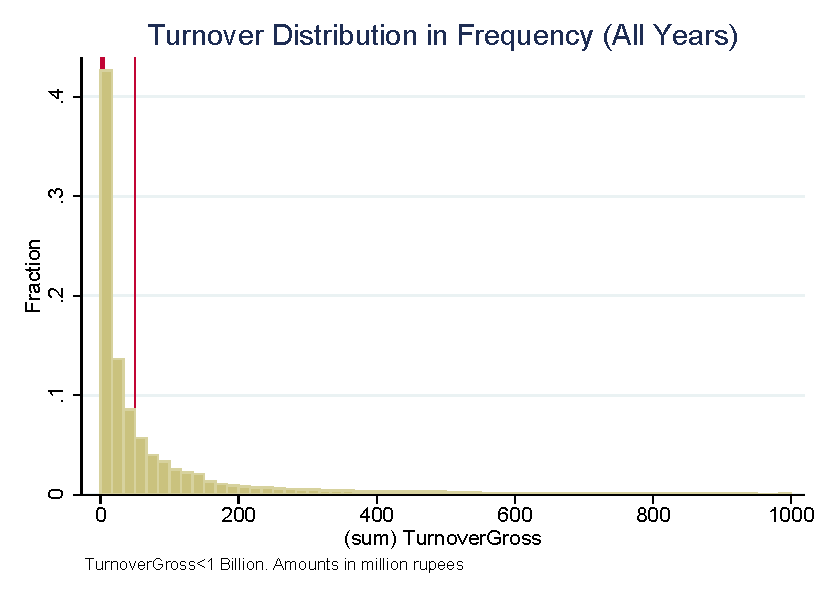
\includegraphics[width=1\textwidth]{graphs/TurnoverDistribution_Fraction_WeaklyPositive} 
 \floatfoot{\footnotesize  Notes: The figure shows the (relatively smooth) distribution of the firms according to their revenue in our sample, combining the samples from each of the years in our analysis (fiscal years 2010/11-2014/15). The x-axis shows the reported firm revenue, while the y-axis shows the corresponding frequency of the firms with the reported revenue shown on the x-axis.}
 % \begin{tablenotes}[flushleft, normal]
%\footnotesize Notes: The figure shows the (relatively smooth) distribution of the firms according to their revenue in our sample, combining the samples from each of the years in our analysis (fiscal years 2010/11-2014/15). The x-axis shows the reported firm revenue, while the y-axis shows the corresponding frequency of the firms with the reported revenue shown on the x-axis.
 % \end{tablenotes}
\end{figure}

We use the form 16 data described in \cref{sec:1-data} and \cref{subsec:1-data-returns} for our analysis. Since all thresholds of interest are defined on annual levels, if a firm is filing multiple returns in a given financial year, we aggregate the values at the financial year level. We have 5 years of tax returns from the state of Delhi, India from the fiscal year 2010-11 until the fiscal year 2014-15.


\subsection{Bunching at Thresholds}
\label{subsec:3-methodology-bunching}
Throughout our bunching analysis, we focus on the effects in the vicinity of each of the thresholds. We divide firms into bins of \rupee30,000 around the low (annual firm revenue of \rupee1 million \textasciitilde{} \$15,000) and the middle thresholds (annual revenue of \rupee5 million \textasciitilde{} \$77,000). Similarly, we divide the firms into bins of \rupee300,000 around the high threshold (annual firm revenue of \rupee50 million \textasciitilde{} \$770,000). 

The lower excluded area, starting at $R_{1}$ to the left of a given threshold and ending at the threshold $T$, features a discontinuous
increase in the distributions of firms right before the threshold. The upper excluded area, starting at the threshold $T$ and ending
at $R_{2}$ to the right of a given threshold, features a missing mass in the number of firms immediately after the threshold. For each
threshold, we visually observe the discontinous increase in the number of firms before the threshold and use this visual observation to find the value of $R_{1}$. We use the convergence method, as described by \citet{kleven2013using}, to find the values of $R_{2}$ for each of the thresholds. Specifically, we choose the value of $R_{2}$ such that the area above the counterfactual distribution between $R_{1}$ and $T$, and the area below the counterfactual distribution between $T$ and $R_{2}$ are approximately equal.

As a proxy estimate of the counterfactual distribution, we draw a fitted fourth-degree polynomial across all observations, excluding
the lower and upper excluded area, to the left and to the right of a given threshold. We run the following regression to estimate the
smooth polynomial: 

\begin{equation}
  \label{eq:main}  
  C_{j}=\sum_{i=1}^{4}\beta_{i}(B_{j})^{i}+\varepsilon_{j},\forall B_{j}\leq R_{1}\&B_{j}\geq R_{2},
\end{equation}
where $C_{j}$ denotes the count of firms in a given bin $B_{j}$, $T$ denotes the threshold, $R_{1}$ denotes the beginning of the lower excluded area range (before the threshold), and $R_{2}$ denotes the end of the upper excluded area range (after the threshold). Once we obtain the estimates from \cref{eq:main}, we then use the predicted counterfactual in the excluded range as well, and predict the counterfactual number of firms as follows:

\begin{equation}
  \label{eq:counterfactual}  
  \hat{C}_{j}=\sum_{i=1}^{4}\beta_{i}(B_{j})^{i}
\end{equation}

We then use the estimated counterfactual to estimate the bunching in the lower excluded area (to the left of the threshold), as follows:
\begin{equation}
  \label{eq:bunching}
  b=\frac{\sum_{i\epsilon S}(C_{i}-\hat{C}_{i})}{\hat{C}_{lowerexcluded}},
\end{equation}
where $S$ denotes the set of values $i$, for which the bins $B_{i}$ are in the lower excluded area, namely: $S=\{i\epsilon\mathbb{N}|B_{i}\epsilon[T-R_{1},T]$. The bunching estimate is thus the estimate of the excess mass in the distribution of firms before the threshold relative to the counterfactual distribution of firms, as a share of the counterfactual distribution of firms in the lower excluded area. In particular the latter value, $\hat{C}_{lowerexcluded}$, is calculated as a weighted average of the counterfactual in the lower excluded area, weighted by the distance of the actual count of firms from the counterfactual distribution, as follows: 
\begin{equation}
  \label{eq:lowerexcluded}
  \hat{C}_{lowerexcluded}=\sum_{i\epsilon S}\mu_{i}\hat{C_{i},}
\end{equation}
where $\mu_{i}$ is the weight of each bin $i$, constructed as follows:

\begin{equation}
  \label{eq:weight}
  \mu_{i}=\frac{C_{i}-\hat{C}_{i}}{\sum_{i\epsilon S}(C_{i}-\hat{C}_{i})}
\end{equation}

We represent the counterfactual distribution of firms with a solid red line in all of the figures showing bunching, while we show the
values of $R_{1}$ and $R_{2}$ using the vertical red dashed lines (refer to \cref{fig:LowestThreshold}, \cref{fig:MiddleThreshold}, and \cref{fig:HighestThreshold}).

\subsection{VAT Revenue Loss to the Tax Authority}
\label{subsec:3-methodology-revenue-loss}
To calculate the tax revenue implications of firm level bunching to avoid increased compliance costs, we need to assume that the firms in the lower excluded area (the excess mass of firms below the threshold), and the firms in the upper excluded area (the missing mass above the threshold) are directly comparable in terms of their unobservable characteristics - apart from their reported revenue and the VAT they remit. We then determine the revenue implication of the threshold regulation as follows. First, we calculate the difference in the average VAT remitted by firms in the upper excluded area and the VAT remitted by firms in the lower excluded area. We then multiply the difference in the average VAT remitted per firm with the extra bunching density, where $B=\sum_{i\epsilon S}(C_{i}-\hat{C}_{i})$. The revenue implication, $R$, is thus calculated as follows:
\begin{equation}
  \label{eq:revenue-implication}
  R=(VAT_{above}^{mean}-VAT_{below}^{mean})*B
\end{equation}

\subsection{No Benefits to More Information}
\label{subsec:3-methodology-more-information}
One question related to the VAT reporting thresholds is why the tax authority might be interested in getting more frequent VAT reports from firms. We test whether the tax authority benefits from the firms providing more frequent information by receiving higher VAT collections when the firms provide more frequent information. We proceed as follows: First, we group all data together, so that we have a pool of observations covering 2010-2015. We then normalize the VAT collected relative to the size of the firm in terms of its revenues, and run the following regression for firm $i$ in year $j$:
\begin{equation}
  (VAT/Revenue)_{i,j}=\alpha+\beta\cdot NumberReports_{i,j}+\phi_{j}+\phi_{i}+\epsilon_{i,j},
\end{equation}
where $VAT/Revenue$ is the ratio of a firm- and year-specific VAT remitted and the reported firm revenue, $\alpha$ is a constant, $NumberReports$ is the annual number of reports filed by the firm given its reported firm size, $\phi_{i}$ and $\phi_{j}$ are the firm and the year fixed effects, respectively (if included in the regression specification, as shown in \cref{tab:number-reports-regressions}), and $\epsilon$ are the heterogeneity robust standard errors.

We additionally test the responsiveness of the VAT collected as a share of revenue to the annual number of submitted reports by regressing the $VAT/Revenue$ ratio on each of the reporting categories, while having the annual reporting as the omitted category. The regression specification for a firm $i$ in year $j$ is then:

\begin{equation}
  (VAT/Revenue)_{i,j}=\alpha+\sum_{c=semiannual}^{monthly}\beta_{c}\cdot c+\phi_{j}+\phi_{i}+\epsilon_{i,j},
\end{equation}

where $VAT/Revenue$ is the ratio of a firm- and year-specific VAT remitted as a share of the reported firm revenue, $\alpha$ is a constant, $c$ can take three values: $semiannual$ is a dummy variable equal to 1 if the firm filed the VAT reports at a semiannual level in a given year, $quarterly$ is a dummy variable equal to 1 if the firm filed the VAT reports at a quarterly level in a given year, $monthly$ is a dummy variable equal to 1 if the firm filed the VAT reports at a monthly level in a given year, $\phi_{i}$ and $\phi_{j}$ are the firm and the year fixed effects, respectively (if included in the regression specification, as shown in \cref{tab:filing-category-regressions}, and $\epsilon$ are the heterogeneity robust standard errors.

Using these regression specifications, we can then estimate the relationship between the number of annually filed reports (or the given reporting categories) and the amount of VAT remitted (relative to the firms' reported revenue) using simple OLS regressions.

\subsection{Social Welfare Analysis}
\label{subsec:3-methodology-welfare-analysis}
We conduct a very simple back of the envelope social welfare analysis. In particular, we recognize that the overall welfare change in our context depends on the sum of the tax authority's revenue losses from the threshold policy, and the easing of compliance costs incurred by the firms in our sample due to the lower filing frequencies that these firms are now required to abide by. Therefore, we recognize that we can calculate the minimum implicit compliance subsidy needed to be given by the tax authority to the firms in a given reporting category in order to at least equalize the revenue losses stemming from the bunching behavior by the firms. If the actual compliance costs for the filing for those firms are higher than the calculated minimum implied subsidies, the overall welfare change stemming from the policy is likely to be positive \textit{net of implicit compliance subsidies}, despite the revenue losses to the tax authority due to the bunching behavior.

%- while not considering the potential compliance spillovers - Not clear what spillovers are we referring to.

We thus calculate the implicit subsidies at each threshold $i$ in the following manner, using the values of revenue losses, $R$, calculated as explained in the subsection \ref{subsec:3-methodology-revenue-loss}:

\begin{equation}
ImplicitSubs_i = R_i / n_j,
\end{equation}

where $n_j$ is the number of firms in the reporting category $j$ below a given threshold $i$. This implies that for the low threshold, we divide the revenue losses stemming from the threshold by the number of firms reporting and paying VAT at an annual level. For the middle threshold, we divide the revenue losses stemming from the threshold by the number of firms reporting and paying VAT at a bi-annual level. Likewise, for the high threshold, we divide the revenue losses stemming from the threshold by the number of firms reporting and paying VAT at a quarterly level. 

We then evaluate whether the implicit subsidies needed to equalize the revenue losses are lower than the likely compliance costs incurred by firms reporting and paying VAT at a certain level of frequency.

\begin{figure}[ht!]
  \centering
  \subfloat[Bunching in Year 1]{
    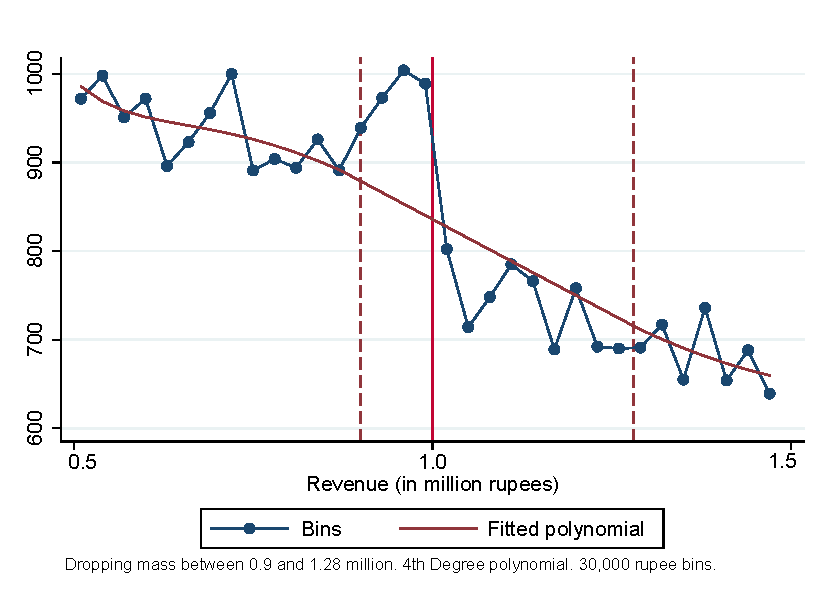
\includegraphics[width=55mm]{graphs/BunchingYear1_1Million_Degree4_30000}
    \label{fig:LowestThreshold-A}
  }
  \subfloat[Bunching in Year 2]{
    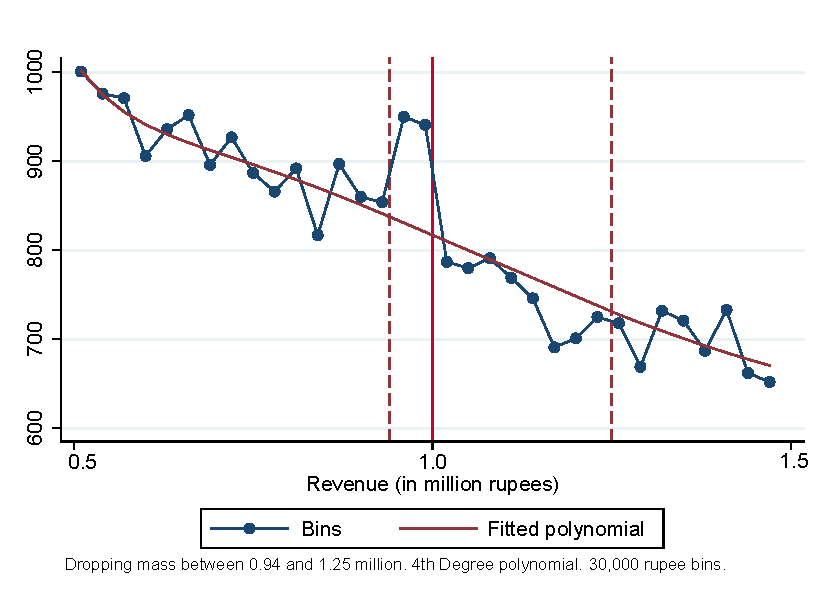
\includegraphics[width=55mm]{graphs/BunchingYear2_1Million_Degree4_30000}
    \label{fig:LowestThreshold-B}
  }
  \hspace{0mm}
  \subfloat[No Bunching in Year 3]{
    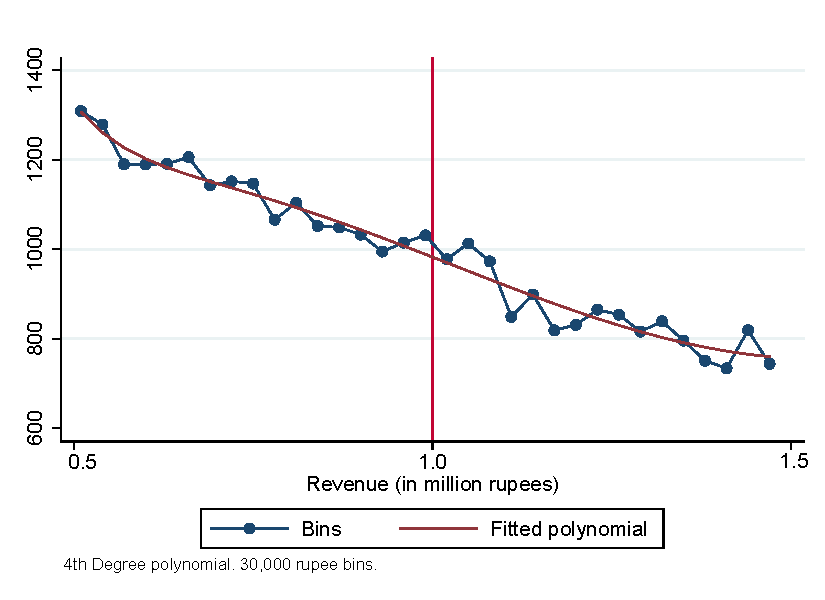
\includegraphics[width=55mm]{graphs/BunchingYear3_1Million_Degree4_30000}
    \label{fig:LowestThreshold-C}
  }
  \subfloat[No Bunching in Year 4]{
    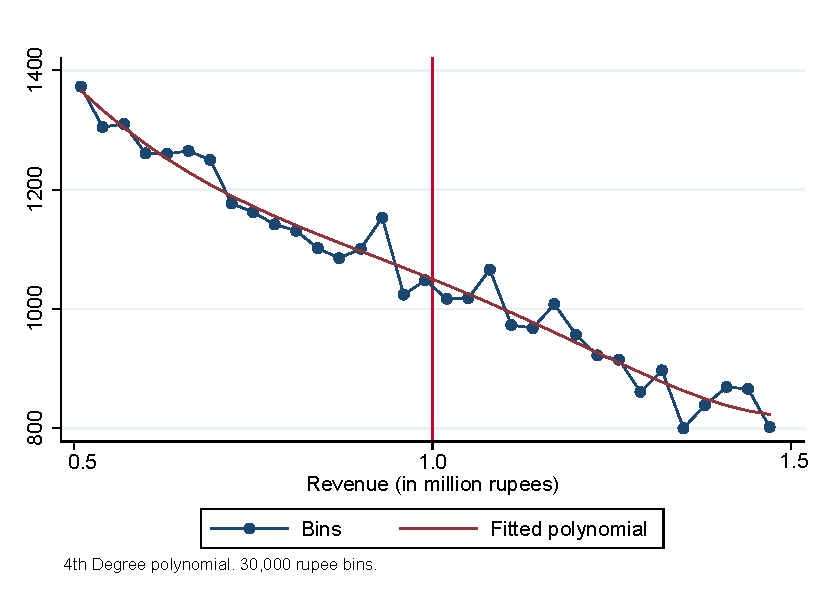
\includegraphics[width=55mm]{graphs/BunchingYear4_1Million_Degree4_30000}
    \label{fig:LowestThreshold-D}
  }
  \hspace{0mm}
  \subfloat[No Bunching in Year 5]{   
    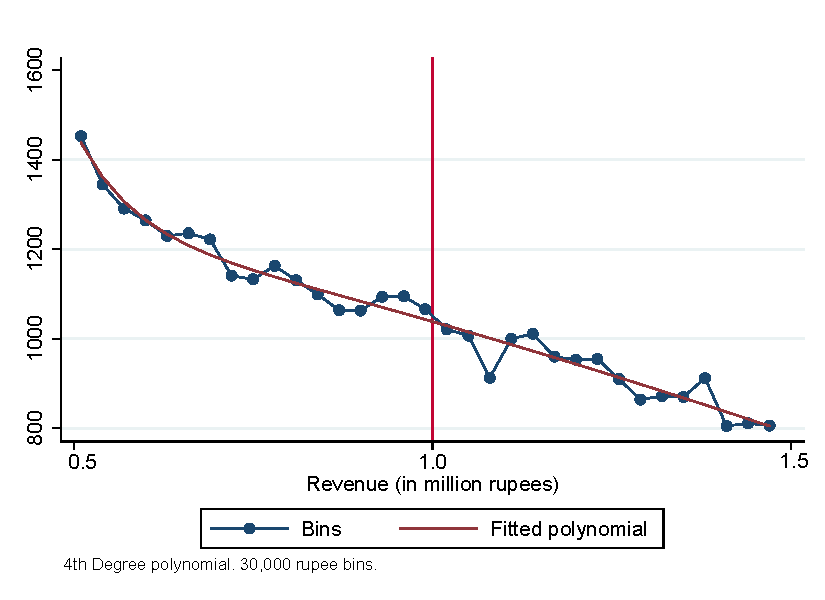
\includegraphics[width=55mm]{graphs/BunchingYear5_1Million_Degree4_30000}
    \label{fig:LowestThreshold-E}
  }
  \caption{Firm Revenue Distribution at the Low Threshold}
  \label{fig:LowestThreshold}
  \floatfoot{\footnotesize Notes: The figure shows the distribution of the firms around the low threshold (\rupee1 million), for each of the years in our data (year 1: fiscal year 2010/11 to year 5: fiscal year 2014/15). Panels A and B show the bunching behavior by the firms for the years (year 1 and 2) with differential, size-dependent requirements of VAT filing, while panels C, D and E document that there is no bunching behavior, with the distribution of firms being smooth around the threshold once the differential reporting requirement is done away with (years 3-5).}
\end{figure}


\section{Results}
\label{sec:3-results}
In this section we describe the results obtained using the methodologies detailed in the previous section. We first discuss the results of estimating the excess bunching at the relevant VAT filing thresholds. The second subsection discusses the calculation of the VAT revenue loss to the tax authority due to the existence of the arbitrary VAT filing thresholds. The third subsection shows that there are no apparent revenue benefits to the tax authority of more frequent information provision by the firms. The fourth subsection concludes by providing the relevant welfare analysis of the size-dependent VAT filing policy.

\subsection{Bunching at Thresholds}
\label{subsec:3-results-bunching}
This section discusses the results of estimating the excess bunching at each of the VAT filing thresholds according to the methodology described in the \cref{subsec:3-methodology-bunching}.

The low threshold, set at the revenue of \rupee1 million, was relevant for the size-dependent VAT filing policy in years 1 and 2 (2010-11 and 2011-12) and mandated the change of return filing from an annual to a bi-annual frequency. \Cref{fig:LowestThreshold-A,fig:LowestThreshold-B} show that such policy resulted in excess bunching at the threshold, with the bunching estimates of 0.5 for year 1, and 0.28 for year 2, respectively. In years 3, 4, and 5, the policy was discontinued, and all the firms around the threshold were required to file their VAT reports on a quarterly basis. As \cref{fig:LowestThreshold-C,fig:LowestThreshold-D,fig:LowestThreshold-E} illustrate, there was - in contrast to years 1 and 2 - no excess bunching around the low threshold in the later years.

\begin{figure}[ht!]
  \centering
  \subfloat[Bunching in Year 1]{
    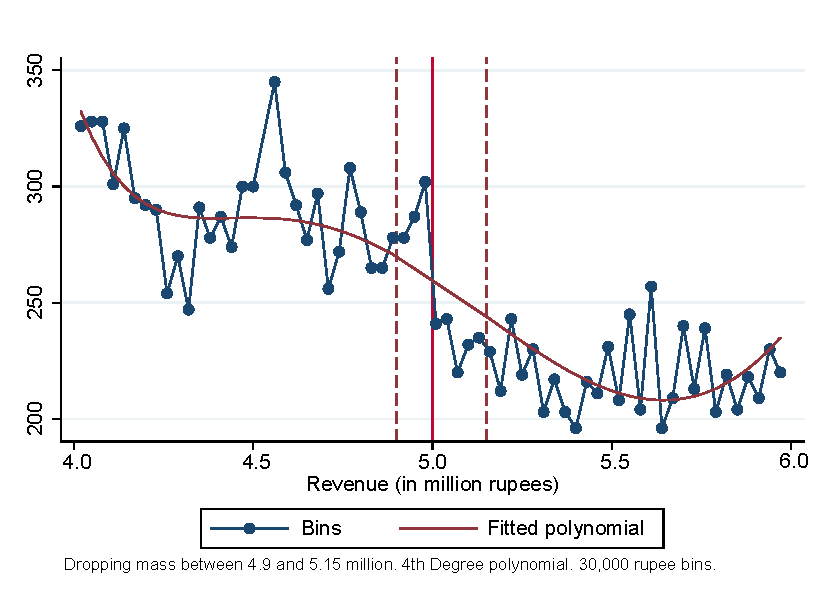
\includegraphics[width=55mm]{graphs/BunchingYear1_5Million_Degree4_30000}
    \label{fig:MiddleThreshold-A}
  }
  \subfloat[Bunching in Year 2]{
    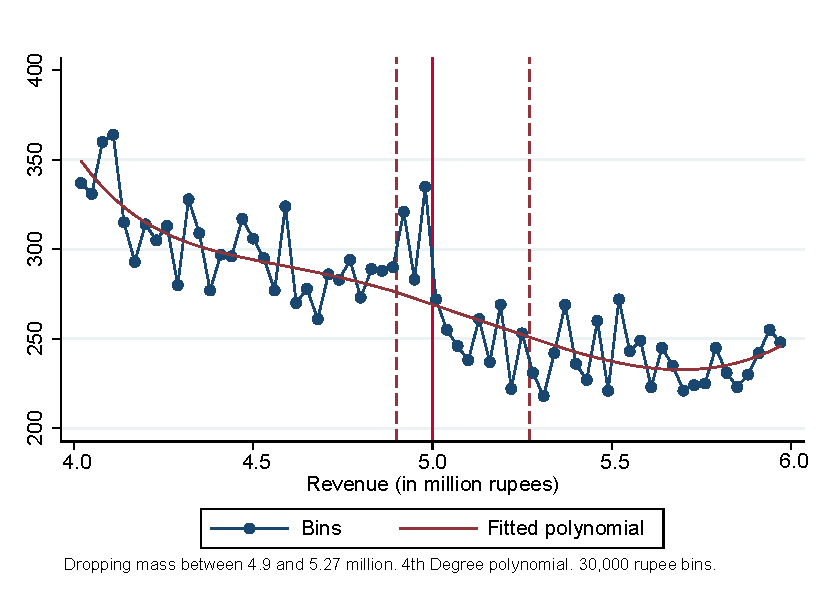
\includegraphics[width=55mm]{graphs/BunchingYear2_5Million_Degree4_30000}
    \label{fig:MiddleThreshold-B}
  }
  \hspace{0mm}
  \subfloat[No Bunching in Year 3]{
    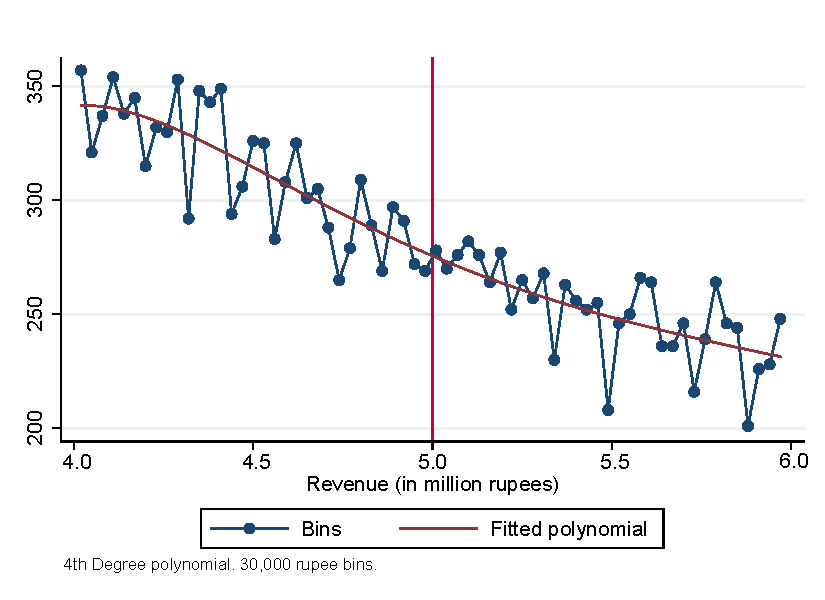
\includegraphics[width=55mm]{graphs/BunchingYear3_5Million_Degree4_30000}
    \label{fig:MiddleThreshold-C}
  }
  \subfloat[No Bunching in Year 4]{
    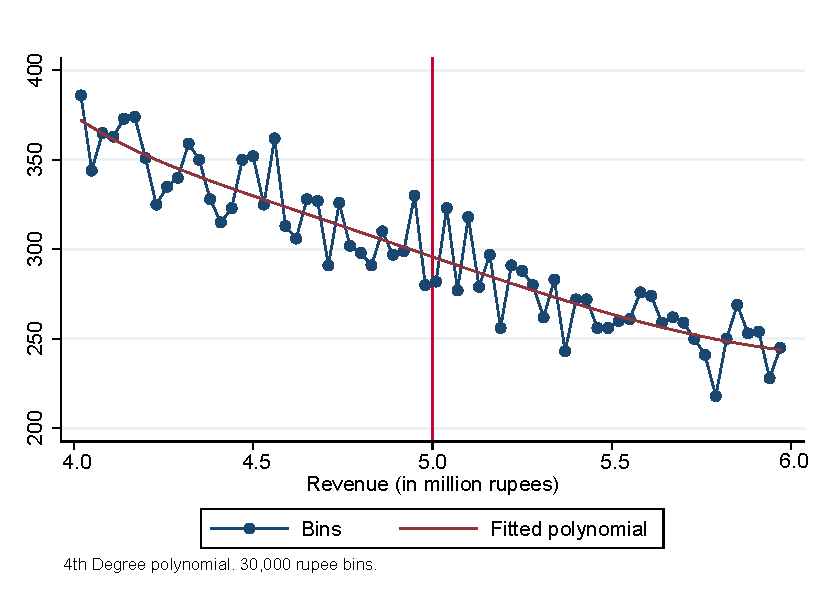
\includegraphics[width=55mm]{graphs/BunchingYear4_5Million_Degree4_30000}
    \label{fig:MiddleThreshold-D}
  }
  \hspace{0mm}
  \subfloat[No Bunching in Year 5]{   
    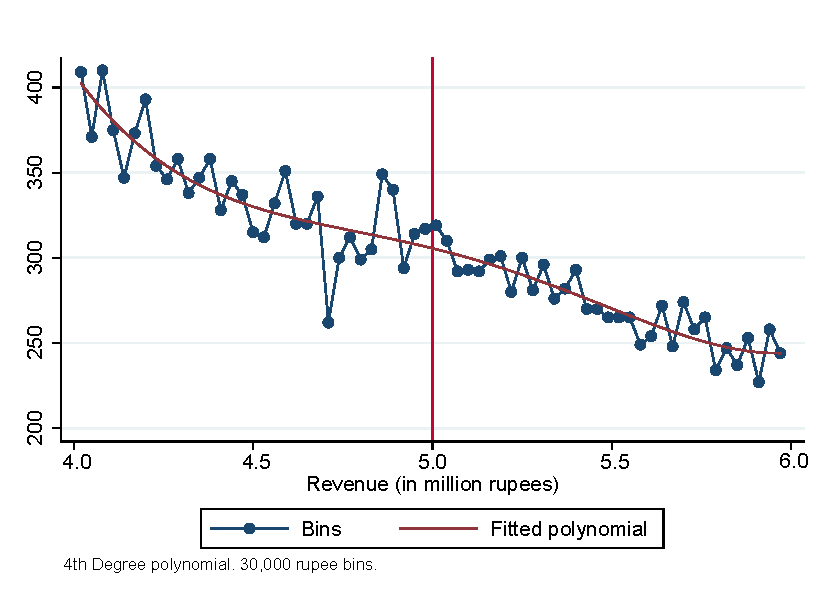
\includegraphics[width=55mm]{graphs/BunchingYear5_5Million_Degree4_30000}
    \label{fig:MiddleThreshold-E}
  }
  \caption{Firm Revenue Distribution at the Middle Threshold}
  \label{fig:MiddleThreshold}
  \floatfoot{\footnotesize Notes: The figure shows the distribution of the firms around the middle threshold (\rupee5 million), for each of the years in our data (year 1: fiscal year 2010/11 to year 5: fiscal year 2014/15). Panels A and B show the bunching behavior by the firms for the years (year 1 and 2) with differential, size-dependent requirements of VAT filing, while panels C, D and E document that there is no bunching behavior, with the distribution of firms being smooth around the threshold once the differential reporting requirement is done away with (years 3-5).}
 \end{figure}

The middle threshold, set at the revenue of \rupee5 million, mandated the change of return filing from a bi-annual to a quarterly frequency in years 1 and 2 (2010-11 and 2011-12). Instead of filing the VAT returns twice a year, firms with the reported revenue above \rupee5 million in the previous year were required to file their reports four times a year. \Cref{fig:MiddleThreshold-A,fig:MiddleThreshold-B} show that such a size-dependent policy resulted in a significant bunching, with bunching estimates equaling 0.34 and 0.43, for years 1 and 2, respectively. \Cref{fig:MiddleThreshold-C,fig:MiddleThreshold-D,fig:MiddleThreshold-E} further show that such bunching disappears, with a much smoother distribution of reported firm revenues, once the threshold policy was done away with in years 3, 4, and 5.

\begin{figure}[ht!]
  \centering
  \subfloat[Bunching in Year 1]{
    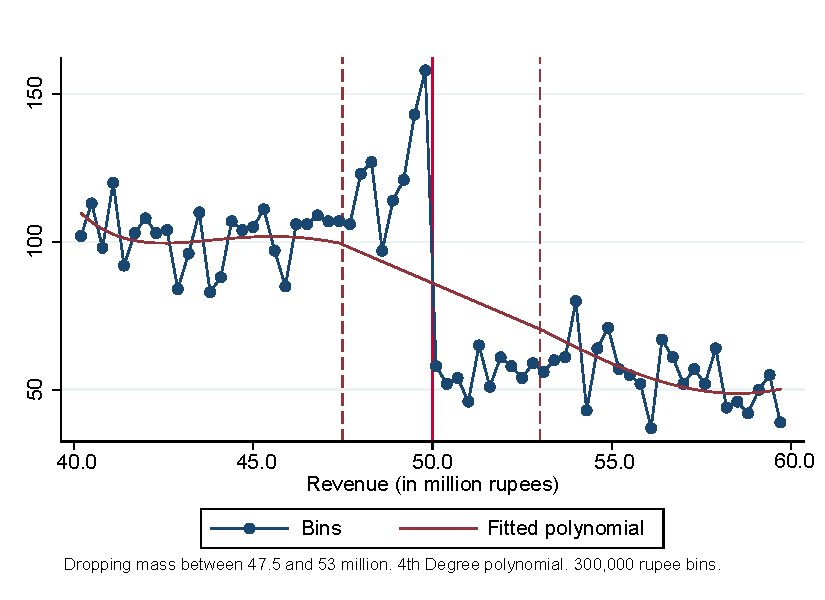
\includegraphics[width=55mm]{graphs/BunchingYear1_50Million_Degree4_3lac}
    \label{fig:HighestThreshold-A}
  }
  \subfloat[Bunching in Year 2]{
    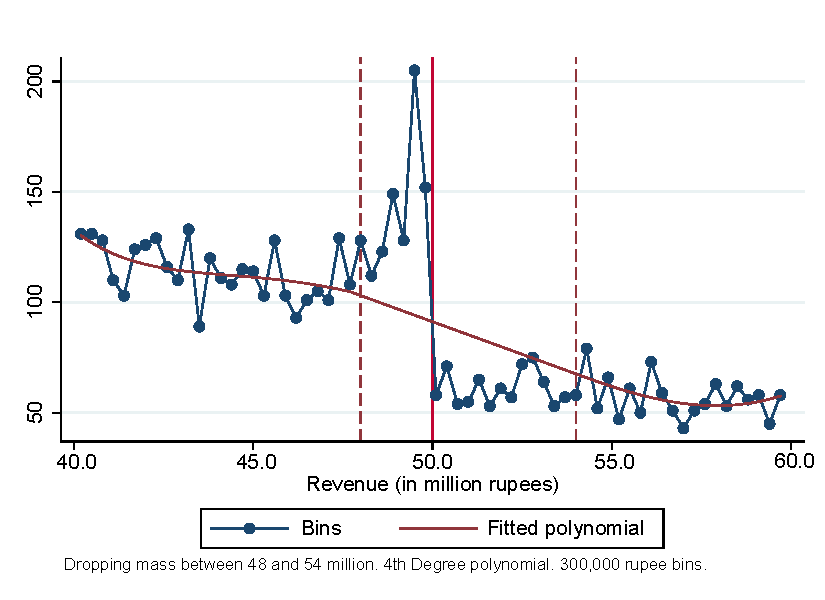
\includegraphics[width=55mm]{graphs/BunchingYear2_50Million_Degree4_3lac}
    \label{fig:HighestThreshold-B}
  }
 \hspace{0mm}
  \subfloat[Bunching in Year 3]{
    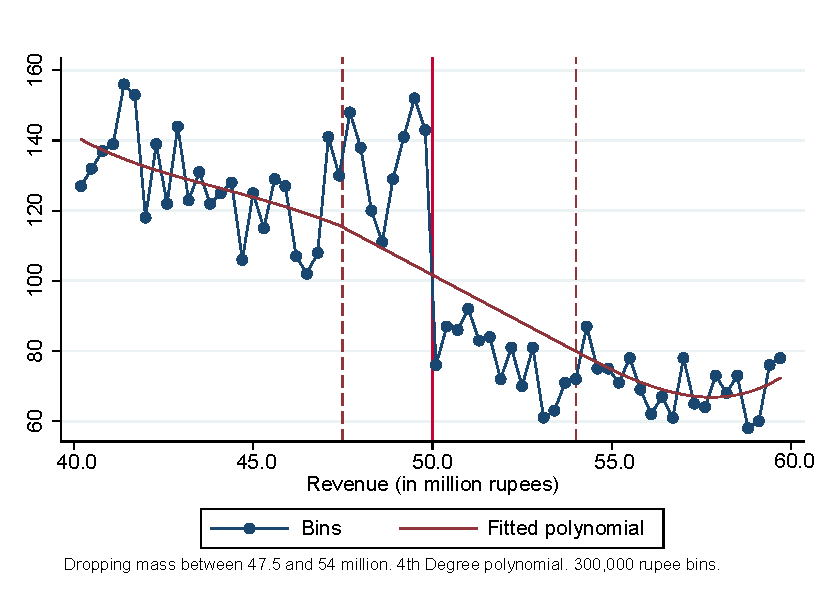
\includegraphics[width=55mm]{graphs/BunchingYear3_50Million_Degree4_3lac}
    \label{fig:HighestThreshold-C}
  }
  \subfloat[No Bunching in Year 4]{
    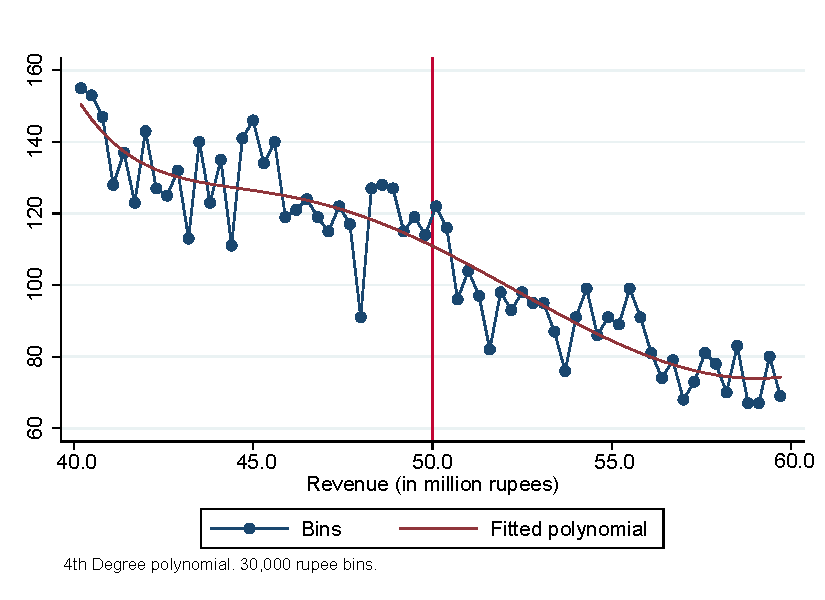
\includegraphics[width=55mm]{graphs/BunchingYear4_50Million_Degree4_3lac}
    \label{fig:HighestThreshold-D}
  }
  \hspace{0mm}
  \subfloat[No Bunching in Year 5]{   
    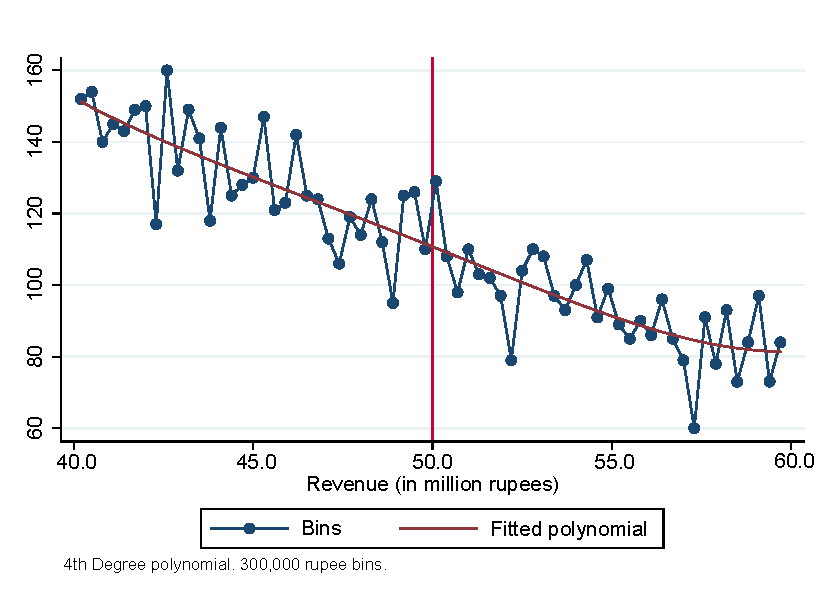
\includegraphics[width=55mm]{graphs/BunchingYear5_50Million_Degree4_3lac}
    \label{fig:HighestThreshold-E}
    }
  \caption{Firm Revenue Distribution at the High Threshold}
  \label{fig:HighestThreshold}
  \floatfoot{\footnotesize Notes: The figure shows the distribution of the firms around the high threshold (\rupee50 million), for each of the years in our data (year 1: fiscal year 2010/11 to year 5: fiscal year 2014/15). Panels A-C show the bunching behavior by the firms for the years (years 1, 2, and 3) with differential, size-dependent requirements of VAT filing, while panels D and E document that there is no bunching behavior, with the distribution of firms being smooth around the threshold once the differential reporting requirement is done away with (years 4 and 5). }
\end{figure}

The highest threshold, set at the revenue of \rupee50 million, mandated the change of return filing from a quarterly frequency to a monthly frequency in years 1, 2, and 3 (2010-11 to 2012-13). In these years, the firms with the reported revenue greater than \rupee50 million, in the previous year, had to file VAT returns twelve times a year compared to firms just below the threshold, which had to file VAT returns four times a year. \Cref{fig:HighestThreshold-A,fig:HighestThreshold-B,fig:HighestThreshold-C} again indicate substantial bunching due to such filing threshold, with bunching estimates equaling 2.6, 2.98, and 1.87, in years 1, 2, and 3, respectively. \Cref{fig:HighestThreshold-D,fig:HighestThreshold-E} show that after the threshold policy was done away with in years 4 and 5 - with all firms now filing the VAT reports on a quarterly basis - the distribution of reported revenues becomes much smoother, with no bunching at the relevant threshold of \rupee50 million. This indicates that the observed bunching indeed occurs due to the filing policy.

Within each of the thresholds, we see that the bunching occurs at approximately the same magnitude. For the low threshold, we see a decrease of bunching in the second year; for the middle threshold, we see a slight increase in the second year bunching; for the high threshold, we see an increase in bunching from year 1 to 2, followed by a decrease in bunching in year 3. Assuming that the level of bunching is a proxy for actual compliance costs incurred by firms, \cref{fig:ComplianceCosts} uses these bunching estimates to track the compliance costs across different revenue sizes and plots the bunching estimates on the y-axis versus the revenue sizes for the relevant thresholds on the x-axis. While compliance costs seem to remain more or less at the same level across the low and middle threshold, we see a sharp increase in the apparent compliance costs at the high threshold. This implies that compliance costs of a differential VAT reporting policy are generally increasing with the reported revenue.

\begin{figure}[ht!]
  \caption{Distribution of Compliance Costs by Revenue Size}
  \label{fig:ComplianceCosts}
  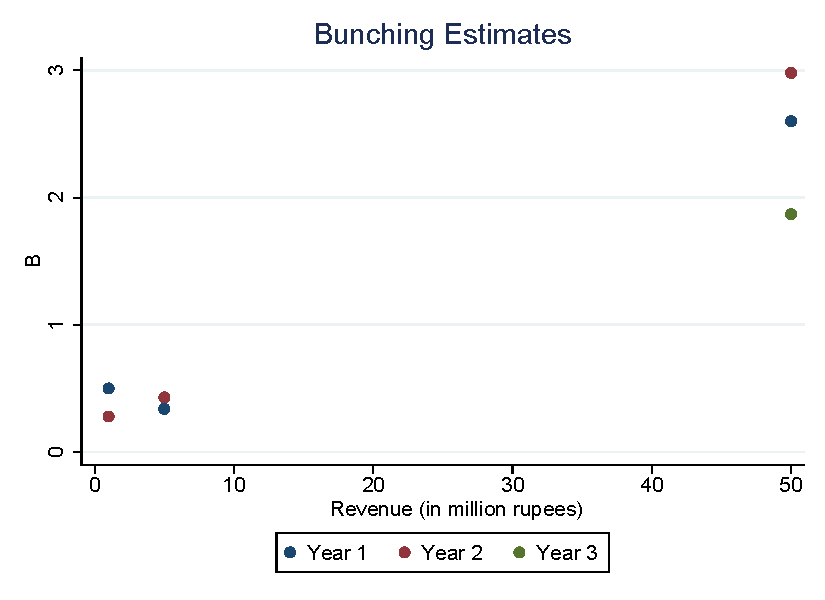
\includegraphics[width=0.8\textwidth]{graphs/BunchingEstimates} 
  \floatfoot{\footnotesize Notes: The figure shows the bunching estimates (on the y-axis) against the reported revenue at each of the thresholds, for which the bunching is estimated. The figure provides an indication of increasing compliance costs with the size of the reported revenue thresholds.}
\end{figure}


\subsection{VAT Revenue Loss to the Tax Authority}
\label{subsec:3-results-revenue-loss}
This section discusses the calculation of the VAT revenue loss to the tax authority due to the differential, size-dependent filing policy according to the methodology described in the \cref{subsec:3-methodology-revenue-loss}.

We compare the VAT contributions of firms in the bunching region below and the region above the threshold. \Cref{tab:VAT-revenue-lost} shows that the revenue losses are substantial. For the low threshold, the losses amount to nearly \rupee900,000 in year 1, and to nearly \rupee500,000 in year 2. These amounts are, respectively, 2.3\% and 1.8\% of the bunchers' (all firms just below the threshold) total VAT contributions, therefore presenting a substantial loss of VAT revenues to the tax authority. For the middle threshold, the losses are generally less substantial, amounting to above \rupee700,000 in year 1, and above \rupee100,000 in year 2. These amounts respectively equal 1.8\% and 0.03\% of the bunchers' total VAT contributions in the respective years. The losses are most substantial for the high threshold, amounting to nearly \rupee40,000,000 in year 1, and above \rupee20,000,000 in years 2 and 3. These amounts are also the highest as a share of the bunchers' total VAT contributions, amounting to 8.3\%, 5.2\%,
and 4.2\% in years 1, 2, and 3, respectively. These estimates confirm the findings in \cref{subsec:3-results-bunching} that the bunching is not only the highest, but also the costliest for the high threshold.

\begin{table}[t]
  \begin{threeparttable}
    \caption{VAT Revenue Lost}
    \label{tab:VAT-revenue-lost}
    \begin{tabular}{cccc}
      \hline 
      & \multicolumn{3}{c}{Threshold level}\\
       & Low   & Middle   & High \\ %\tabularnewline
      %\hline 
      Year  & (\rupee1 million)  & (\rupee5 million)  & (\rupee50 million)\tabularnewline
      \hline 
      2010-11  & 886,017  & 730,557   & 38,373,960  \tabularnewline
       & (2.3\%)  & (1.8\%)  & (8.3\%)\tabularnewline
      %\hline 
      2011-12  & 441,600   & 128,150   & 21,862,749 \tabularnewline
       & (1.8\%)  & (0.03\%)  & (5.2\%)\tabularnewline
      %\hline 
      2013-14  &  &  & 22,871,560\tabularnewline
       &  &  & (4.2\%)\tabularnewline
      \hline 
	\end{tabular}
	\begin{tablenotes}[para]
		Notes: Values in Indian rupees. The amounts expressed as a percentage of the bunchers' (i.e. that of firms in the lower excluded area) VAT contributions are in the brackets. The values are calculated as described in the \cref{subsec:3-methodology-revenue-loss}.
	\end{tablenotes}
  \end{threeparttable}
\end{table}


\subsection{No Benefits to More Information}
\label{subsec:3-results-more-information}
This section discusses the regressions looking at the relationship between the \\ VAT/revenue ratio and the frequency of VAT reporting, as discussed in the methodology \cref{subsec:3-methodology-more-information}. \Cref{tab:number-reports-regressions} shows the regression results looking at the relationship between the VAT/revenue ratios and the yearly number of VAT reports. 

\begin{table}[t]
\scalebox{0.95}{
  \begin{threeparttable}
    \caption{VAT Revenue vs. Annual Number of VAT Returns Regressions}
    \label{tab:number-reports-regressions}
    \begin{tabular}{lcccc}
\multicolumn{5}{c}{}\tabularnewline
\hline 
 & (1)  & (2)  & (3)  & (4) \tabularnewline
VARIABLES  & VAT/Revenue  & VAT/Revenue  & VAT/Revenue  & VAT/Revenue \tabularnewline
\hline 
 &  &  &  & \tabularnewline
NumberReports  & -0.000148{*}{*}{*}  & -0.000314{*}{*}{*}  & 0.000474  & 0.000247 \tabularnewline
 & (3.18e-05)  & (0.000100)  & (0.000468)  & (0.000278) \tabularnewline
 &  &  &  & \tabularnewline
Firm FE  & NO  & NO  & YES  & YES \tabularnewline
Time FE  & NO  & YES  & NO  & YES \tabularnewline
 &  &  &  & \tabularnewline
Observations  & 1,038,331  & 1,038,331  & 1,038,331  & 1,038,331 \tabularnewline
No. of firms  & 301,147  & 301,147  & 301,147  & 301,147 \tabularnewline
$R^{2}$  & 0.000  & 0.000  & 0.703  & 0.703 \tabularnewline
\hline 
%\multicolumn{5}{c}{ Robust standard errors, clustered at the firm level, in parentheses}\tabularnewline
%\multicolumn{5}{c}{ {*}{*}{*} p$<$0.01, {*}{*} p$<$0.05, {*} p$<$0.1}\tabularnewline
\end{tabular}
 
    \begin{tablenotes}[para]
      \footnotesize Notes: Robust standard errors, clustered at the firm level, in parentheses. The regression table presents the results of regressions performed according to the methodology described in the \cref{subsec:3-methodology-more-information}. {*}{*}{*} p$<$0.01, {*}{*} p$<$0.05, {*} p$<$0.1.
    \end{tablenotes}
  \end{threeparttable}}
\end{table}

Columns 1 and 2 show that the relationship is strikingly negative without including firm fixed effects in the regression specification, implying that the greater the number of
VAT reports per year, the smaller the VAT/revenue ratio. When including firm fixed effects in the regression specification, as shown by columns 3 and 4, the relationship turns positive but strongly insignificant.

\begin{table}[t]
\scalebox{0.92}{
  \begin{threeparttable}
    \caption{VAT Revenue vs. VAT Filing Categories Regressions}
    \label{tab:filing-category-regressions}
    \begin{tabular}{lcccc}
\multicolumn{5}{c}{}\tabularnewline
\hline 
 & (1)  & (2)  & (3)  & (4) \tabularnewline
VARIABLES  & VAT/Revenue  & VAT/Revenue  & VAT/Revenue  & VAT/Revenue \tabularnewline
\hline 
 &  &  &  & \tabularnewline
SemiAnnualCategory  & -0.00685{*}{*}{*}  & -0.00685{*}{*}{*}  & 0.00521  & 0.00516 \tabularnewline
 & (0.000206)  & (0.000206)  & (0.00782)  & (0.00778) \tabularnewline
QuarterlyCategory  & -0.00312{*}  & -0.00677{*}{*}{*}  & 0.00696  & 0.00606 \tabularnewline
 & (0.00162)  & (0.000313)  & (0.00823)  & (0.00819) \tabularnewline
MonthlyCategory  & -0.00541{*}{*}{*}  & -0.00713{*}{*}{*}  & 0.00670  & 0.00546 \tabularnewline
 & (0.000286)  & (0.000999)  & (0.00819)  & (0.00717) \tabularnewline
 &  &  &  & \tabularnewline
Firm FE  & NO  & NO  & YES  & YES \tabularnewline
Time FE  & NO  & YES  & NO  & YES \tabularnewline
 &  &  &  & \tabularnewline
Observations  & 1,038,331  & 1,038,331  & 1,038,331  & 1,038,331 \tabularnewline
No. of firms  & 301,147  & 301,147  & 301,147  & 301,147 \tabularnewline
$R^{2}$  & 0.000  & 0.000  & 0.703  & 0.703 \tabularnewline
\hline 
%\multicolumn{5}{c}{Robust standard errors, clustered at the firm level, in parentheses}\tabularnewline
%\multicolumn{5}{c}{Annual reporting is the omitted category. {*}{*}{*} p$<$0.01, {*}{*}
%p$<$0.05, {*} p$<$0.1}\tabularnewline
\end{tabular}
 
    \begin{tablenotes}[para]
	    \footnotesize Notes: Robust standard errors, clustered at the firm level, in parentheses. Annual reporting is the omitted category. The regression table presents the results of regressions performed according to the methodology described in the \cref{subsec:3-methodology-more-information}. {*}{*}{*} p$<$0.01, {*}{*}
p$<$0.05, {*} p$<$0.1.
    \end{tablenotes}
  \end{threeparttable}}
\end{table}

\Cref{tab:filing-category-regressions} similarly shows the regression results looking at the relationship between the VAT/revenue ratios and different reporting categories, with annual reporting being the omitted category. As columns 1 and 2 show, when not including firm fixed effects, all reporting categories are negatively related to the VAT/revenue ratios compared to those firm-year observations with annual reporting. Once including firm fixed effects in the regression, the estimates turn positive, but again remain strongly insignificant.

Our interpretation of the results of both of the sets of regressions is that greater than annual frequency of VAT reporting does not lead to more VAT being collected, as measured by the VAT/revenue ratios.

\subsection{Social Welfare Analysis}
\label{subsec:3-results-social-welfare}
In this section we discuss the results of the back of the envelope social welfare analysis that we conducted according to the methodology outlined in \cref{subsec:3-methodology-welfare-analysis}. In \cref{tab:implicit-subsidies} we present the calculated implicit subsidies. The implicit subsidies needed to equalize welfare are very low. At the low threshold for year 1 - an implicit welfare equalizing per firm subsidy of \rupee40.77 (less than \$1) implies that the welfare change of reducing the frequency would be negative only in the case that compliance costs borne by a given firm reporting and paying VAT at an annual level would be less than \$1, which is extremely unlikely. The implicit welfare equalizing per firm subsidy for year 2, at the low threshold is even smaller. Similarly, the welfare equalizing subsidies for the middle threshold are comparably low. 

The implicit welfare equalizing subsidies for the high threshold are an order of magnitude higher, ranging from \rupee1327.97 (about \$25) in year 3 to \rupee2990.02 (about \$60) in year 1. The implication of these implicit welfare equalizing per firm subsidies is, however, similar as for the low and the middle thresholds. The actual compliance - that is, filing and paying - costs difference (quarterly level of reporting relative to monthly reporting) associated with VAT of these firms, reporting at a quarterly level is certainly higher than \$60. That means that the tax authority subsidizes these firms by reducing the frequency at which they have to file, and yet increases the social welfare. Put another way, this analysis leads us to conclude that even though the tax authority incurs significant losses due to thresholds, its implicit subsidies to small and medium-sized firms are large enough to overcome the revenue losses.
 
\begin{table}[t]
  \begin{threeparttable}
    \caption{Implicit Welfare Equalizing Per Firm Subsidies from the Thresholds}
    \label{tab:implicit-subsidies}
    \begin{tabular}{cccc}
    \hline 
    & \multicolumn{3}{c}{Threshold level}\\

    & Low threshold  & Middle threshold  & High threshold \\
    Year  & ( \rupee1 million)  & ( \rupee5 million)  & ( \rupee50 million)\tabularnewline
    \hline 
    2010-11  &  40.77  &  14.54  &  2990.02 \\
    2011-12  &  17.31 &  2.55  &  1505.49 \\
    2013-14  &  &  &  1327.97 \\
    \hline 
    \end{tabular}
    \begin{tablenotes}[para]
    	\footnotesize Notes: Values in Indian rupees. The implicit minimum welfare equalizing per firm subsidies are computed according to the methodology in the \cref{subsec:3-methodology-welfare-analysis}
    \end{tablenotes}
  \end{threeparttable}
\end{table}


\section{Conclusion}
\label{sec:conclusion}
In this paper, we identify bunching behavior by firms at the VAT filing thresholds, using an administrative-level dataset from the state of Delhi in India. Our unique dataset along with rich policy variation also enables us to show that the bunching completely disappears when the thresholds are done away with. The bunching is the greatest at the highest threshold indicating that compliance is most costly for those firms. We further show that the VAT revenue losses due to the bunching response by firms are substantial, up to 8.3\% of the bunchers' total VAT contributions in certain years. We also suggest that there may be no benefits to the tax authority from receiving more frequent information through the VAT filing reports. Finally, our social welfare analysis shows that given that the costs of compliance by the firms are likely relatively large, the net-of-implicit-subsidies welfare impact of the thresholds is positive despite the substantial revenue losses to the tax authority.

We note two potential channels through which the firms may bunch: underproduction and underreporting. The first channel, underproduction, would imply that the bunching firms halt their production or sales as soon as they start getting close to the threshold. This channel potentially brings about large welfare losses, not only because of the current reduction in the firm-level profits, but also due to the shift in the long-run growth path of the bunching firms. In the case of such channel being the dominant one, the welfare losses due to the policy (while not considering the implicit subsidies due to the reduced filing frequencies for smaller firms) would be the highest, with real and longer-term consequences in the form of stalled firm growth. The second potential bunching channel encompasses the intentional revenue underreporting by the firms. If such underreporting occurs and is substantial, the welfare losses would occur via the lost tax revenues. One potential sub-channel in the firm revenue underreporting is revenue shifting: in such a case, a portion of the bunching firms illegitimately register a part of their sales for the following filing period in order to avoid passing the relevant reporting threshold. In such a case, the welfare consequences of the policy would be the smallest of the three bunching channel options; the firms would only misreport the current revenues to avoid more frequent filing, but would not affect their actual long term real growth, and would eventually report all of their revenues. In future work, we intend to make progress on identifying which of the potential channels are in play.

\todo[inline, caption={Is this the first time?}]{Conclusion is not the right place to desribe something new for the first time. Verify that channels are being talked about earlier.}
\todo[inline, caption={Revenue shifting unclear}]{How can this shifting happen over multiple years?}

All in all, our analysis shows that firms' compliance costs to the VAT policy are quite large, with unclear benefits of more frequent information and payments being made by the VAT registered firms. Tax authorities should thus aim to reduce the compliance costs, which apparently play a substantial role in the firms' behavior. 